\subsection{Level3.1: パラメータのチューニング}
\subsubsection{最適なパラメータを探すためのアプローチ}
指定された条件下において学習が効率良く行われるパラメータの組み合わせを探
すため、**して**することでパラメータを調整した。

(補足:全パターンを調べても良いし、いくつかのパターンを調べても良いが、
どのような方法で調整したら良いかを考えよう。その上で、自分たちがどのよ
うに取り組んだのか(=アプローチ)を説明しよう。)

\subsubsection{実行結果}

(補足:ボーナスポイントの確認がありますので、シード値10パターンで試した際の収
束に要した学習回数と、その平均回数が分かるように明示してください。)
\begin{table}[htb]
 \begin{center}
  \caption{階層型NNによる文字認識問題の学習に要した回数}
  \label{table:level3}
  \begin{tabular}[htb]{r|l} \hline
   シード値 & 収束した回数 \\ \hline \hline
   100 & hoge \\ \hline
   200 & hoge \\ \hline
   300 & hoge \\ \hline
   400 & hoge \\ \hline
   500 & hoge \\ \hline
   600 & hoge \\ \hline
   700 & hoge \\ \hline
   800 & hoge \\ \hline
   900 & hoge \\ \hline
   1000 & hoge \\ \hline \hline
   10試行の平均値 & hoge \\ \hline
  \end{tabular}
 \end{center}
\end{table}

\begin{figure}[h]
 \begin{center}
  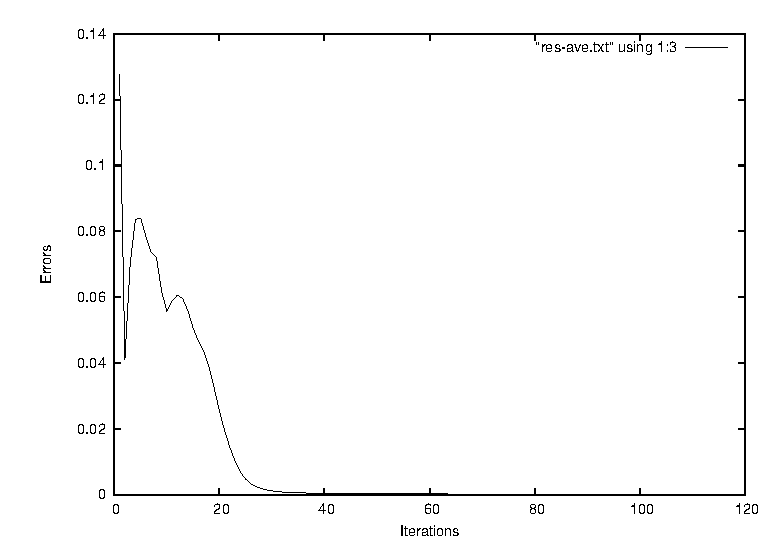
\includegraphics[width=10.0cm]{figs/sample2.eps}
  \caption{重みを更新する様子(平均値)}
  \label{fig:level2}
 \end{center}
\end{figure}


\subsubsection{考察}


